% ============================================================================
% CHAPTER 1: INTRODUCTION
% ============================================================================

\chapter{INTRODUCTION}

\section{OBJECTIVE}

The primary objective of this project is to develop an interpretable deep learning system for the objective detection of Major Depressive Disorder (MDD) from electroencephalogram (EEG) signals. Unlike existing approaches that often report inflated accuracy metrics due to methodological flaws, this system employs rigorous evaluation protocols that reflect real-world clinical deployment scenarios.

\subsection{Primary Objectives}

The first and most significant objective of this work is to design a novel multi-branch deep learning architecture that captures the full complexity of EEG signals associated with depression. This hybrid model combines a Vision Transformer for time-frequency analysis with a Graph Attention Network (GNN) for spatial electrode relationship modeling. The Vision Transformer processes Continuous Wavelet Transform scalograms, enabling the model to learn complex patterns in the time-frequency domain through self-attention mechanisms. Simultaneously, the Graph Attention Network treats the EEG electrode array as a graph structure, where nodes represent individual electrodes and edges encode both spatial proximity and functional connectivity relationships. This dual-branch approach captures complementary information from EEG signals that single-branch architectures inevitably miss, as temporal dynamics and spatial relationships provide orthogonal views of neural activity patterns associated with depression.

The second objective focuses on implementing rigorous Leave-One-Subject-Out (LOSO) cross-validation to ensure that the model is tested exclusively on subjects it has never encountered during training. This validation strategy is critical because it prevents data leakage---a pervasive problem in EEG-based classification research where epochs from the same subject appear in both training and test sets. By ensuring complete subject-level separation, LOSO provides honest performance estimates that accurately reflect the model's true generalization capability and simulate the real clinical deployment scenario where a trained system encounters a completely new patient.

The third objective is to provide multi-level explainability through three complementary methods. Integrated Gradients (IG) attributes model predictions to specific input features by computing path integrals from a baseline to the actual input, revealing which time-frequency regions and electrodes most influence classification decisions. Layer-wise Relevance Propagation (LRP) traces the contribution of each neuron backward through the network, providing a layer-by-layer understanding of how the model processes information. Testing with Concept Activation Vectors (TCAV) enables validation against high-level clinical concepts such as ``frontal alpha asymmetry'' or ``elevated theta power,'' directly testing whether the model has learned established depression biomarkers. Together, these methods ensure that the model's decision-making is transparent and clinically interpretable.

The fourth objective is to validate the model's learned representations against established neurophysiological biomarkers of depression. Through the explainability analysis described above, this project confirms that the model's decision-making aligns with decades of clinical research identifying frontal alpha asymmetry, elevated frontal theta activity, global alpha power reduction, and delta abnormalities as signatures of depression. This validation is essential for clinical acceptance, as it demonstrates that the model learns meaningful neurophysiological patterns rather than spurious correlations or subject-specific artifacts.

\subsection{Secondary Objectives}

Beyond the primary objectives, this project pursues several secondary goals that enhance the system's scientific rigor and practical utility. The system processes raw EEG signals rather than relying on pre-extracted features, maintaining full control over the signal processing pipeline. This approach enables custom preprocessing tailored to depression detection and allows extraction of features specifically designed for the proposed architecture, rather than being constrained by features extracted for other purposes.

The feature extraction methodology employs multi-wavelet Wavelet Packet Decomposition using three complementary wavelet families: Daubechies-4 (db4), Symlet-5 (sym5), and Coiflet-3 (coif3). Each wavelet family offers distinct characteristics in terms of symmetry, vanishing moments, and time-frequency localization, and their combination provides a richer spectral representation than any single wavelet could achieve. This multi-wavelet approach yields 576 features per channel, capturing fine-grained frequency information across the entire EEG spectrum.

For the Transformer branch, the system generates Continuous Wavelet Transform scalograms as two-dimensional time-frequency representations. These 64×128 images encode how spectral content evolves over the 4-second epoch duration, providing the ideal input format for the Vision Transformer architecture. The scalograms are computed using the Complex Morlet wavelet, which offers excellent joint time-frequency resolution for EEG analysis.

From a practical standpoint, the project targets clinically meaningful subject-level accuracy exceeding 85\% on completely unseen subjects---a threshold that represents genuine diagnostic utility rather than inflated metrics from leaky validation. Additionally, the architecture is designed for memory efficiency, capable of training on consumer-grade GPUs with less than 8GB VRAM, making the approach accessible to researchers without access to high-end computing infrastructure.

\section{PROBLEM STATEMENT}

\subsection{Global Burden of Depression}

Major Depressive Disorder represents one of the most significant public health challenges of the 21st century. According to the World Health Organization \cite{who2023depression}, depression affects more than 280 million people worldwide, making it the leading cause of disability globally. The economic burden is equally staggering, with depression costing an estimated \$1 trillion annually in lost productivity across direct healthcare costs, reduced workplace performance, and increased absenteeism. Most tragically, depression is linked to approximately 700,000 suicides each year, representing a preventable loss of life that underscores the urgent need for improved diagnostic and treatment approaches.

\begin{figure}[H]
    \centering
    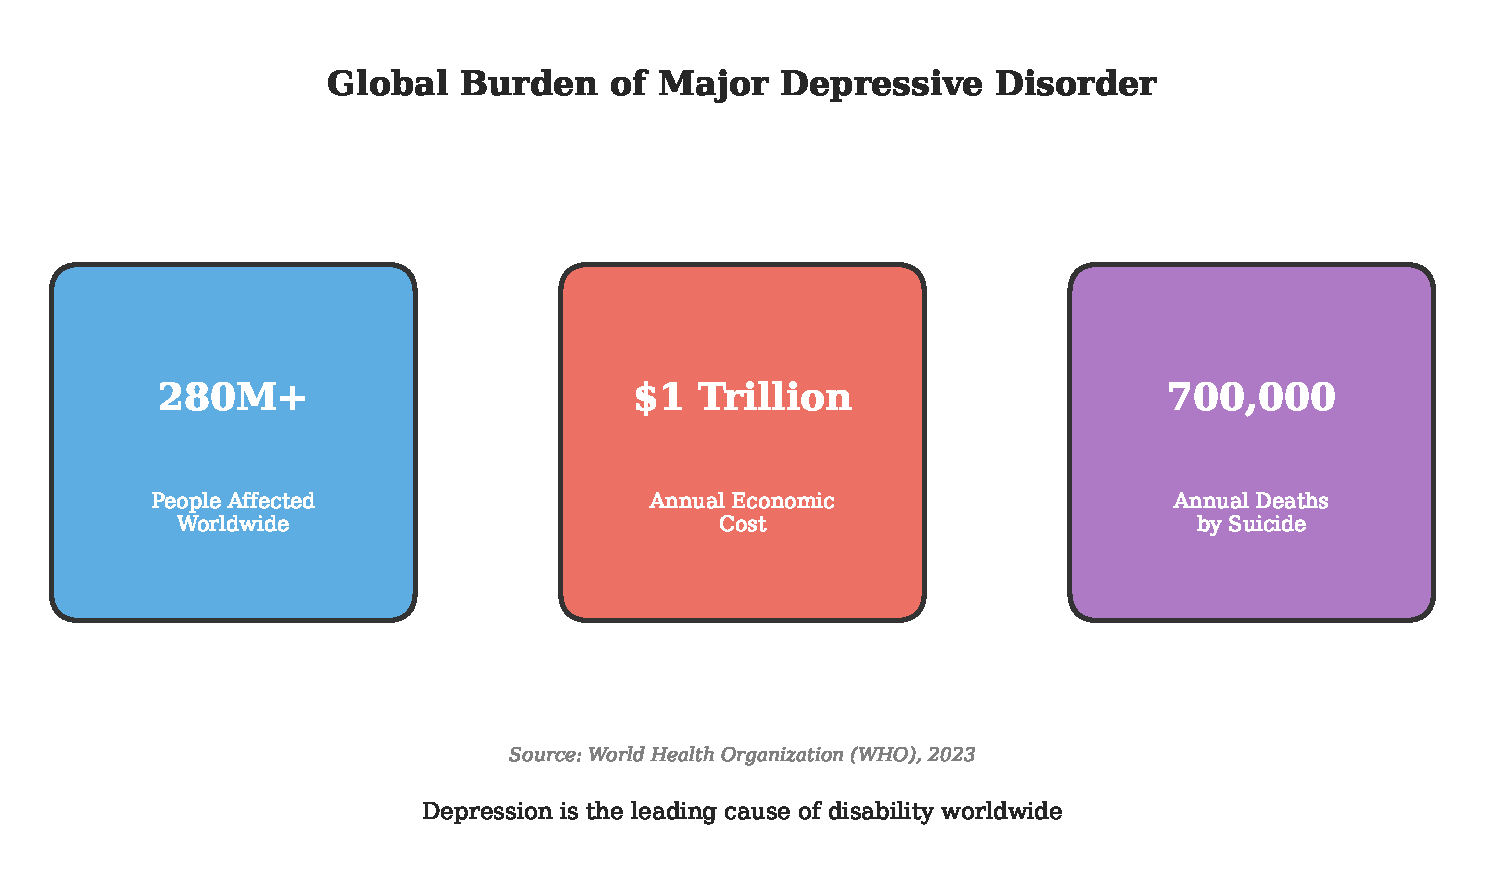
\includegraphics[width=0.85\textwidth]{figures/ch1/fig1_1_depression_statistics.pdf}
    \caption{Global burden of Major Depressive Disorder showing worldwide prevalence, economic impact, and mortality statistics.}
    \label{fig:depression_statistics}
\end{figure}

Despite this enormous burden, the diagnosis of depression remains fundamentally subjective. Clinicians rely primarily on structured interviews and self-reported symptom questionnaires such as the Patient Health Questionnaire-9 (PHQ-9) and Beck Depression Inventory-II (BDI-II). While these tools are clinically validated and widely used, they suffer from several inherent limitations that underscore the pressing need for objective biomarkers that can complement clinical judgment.

\subsection{Limitations of Current Diagnostic Approaches}

Current diagnostic methods for depression face significant challenges that limit their reliability and clinical utility. Inter-rater variability represents a fundamental problem, as different clinicians may arrive at different diagnoses for the same patient. This variability is particularly pronounced in mild-to-moderate cases where symptoms are less clearly defined, and the distinction between normal sadness and clinical depression requires subjective interpretation. Studies have shown that agreement between clinicians on depression diagnosis, even when using structured interviews, falls well short of perfect concordance.

Patient recall bias presents another significant limitation of questionnaire-based assessment. Self-reported instruments depend on patients accurately recalling and reporting their symptoms over the preceding one to two weeks, which is inherently unreliable. Depressed patients may exhibit cognitive symptoms including memory impairment and concentration difficulties that directly compromise their ability to accurately report their own mental state. Furthermore, the retrospective nature of these assessments means that current mood state can color recollection of past symptoms, leading to systematic biases in reporting.

Cultural and language barriers pose additional challenges to standardized assessment. Depression manifests differently across cultures, with some populations expressing psychological distress primarily through somatic symptoms rather than the cognitive and emotional symptoms emphasized in Western diagnostic frameworks. Standardized questionnaires developed and validated in one cultural context may not adequately capture the expression of depression in different populations, leading to systematic underdiagnosis in some groups.

The stigma surrounding mental illness contributes to underreporting of symptoms, as patients may minimize or deny their experiences due to concerns about social judgment, employment consequences, or internalized shame. This is particularly problematic in populations where mental health stigma remains high, and the resulting underreporting leads to delayed or missed diagnoses with corresponding delays in appropriate treatment.

Perhaps most fundamentally, current diagnostic approaches lack objective biomarkers. Unlike many medical conditions that can be confirmed through blood tests, imaging findings, or other physiological measurements, there is no laboratory test that definitively confirms depression. This absence of objective markers means that diagnosis relies entirely on patient report and clinical observation, with all the limitations these subjective assessments entail.

\subsection{EEG as a Potential Biomarker}

Electroencephalography offers a promising avenue for objective depression detection due to several advantageous characteristics that make it well-suited for clinical translation. EEG is entirely non-invasive, requiring only surface electrodes placed on the scalp to record the brain's electrical activity. Unlike invasive procedures or those requiring injection of contrast agents, EEG poses minimal risk to patients and can be repeated as often as clinically necessary without cumulative harm.

From an economic perspective, EEG equipment is significantly less expensive than alternative neuroimaging modalities such as MRI or PET scanners. A clinical-grade EEG system costs a fraction of what MRI installation and maintenance require, making EEG-based diagnostics potentially accessible to a much broader range of clinical settings, including primary care offices and community mental health centers where depression is most commonly encountered.

EEG provides exceptional temporal resolution, capturing neural activity at millisecond timescales that far exceed what is achievable with hemodynamic imaging methods like fMRI. This temporal precision is particularly valuable for depression research, as the neural dynamics associated with emotional processing and cognitive control operate on rapid timescales that EEG can resolve. The ability to track moment-to-moment fluctuations in brain activity provides rich information about the temporal dynamics of neural processing.

Most importantly for this project, decades of research have identified several EEG patterns that are consistently associated with depression and have been replicated across multiple independent studies. These established biomarkers provide a foundation for machine learning approaches and, crucially, offer a means to validate that learned models are capturing clinically meaningful patterns rather than spurious correlations.

\begin{figure}[H]
    \centering
    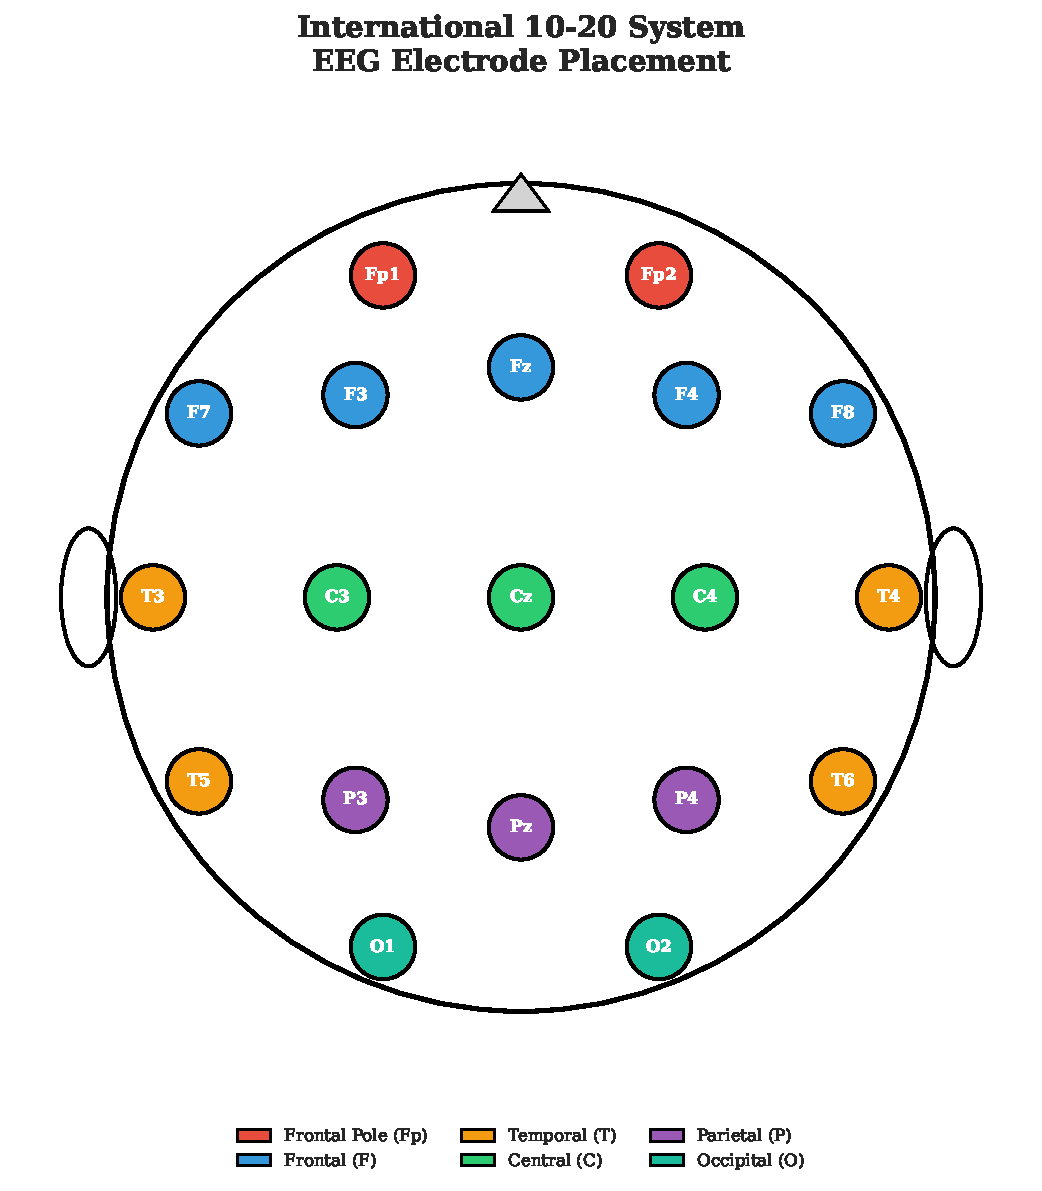
\includegraphics[width=0.75\textwidth]{figures/ch1/fig1_2_electrode_placement.pdf}
    \caption{International 10-20 System for EEG electrode placement showing the 19 standard electrode positions used in this study.}
    \label{fig:electrode_placement}
\end{figure}

Table \ref{tab:eeg_biomarkers} summarizes the established EEG biomarkers associated with depression that have been validated in clinical research. These biomarkers span multiple frequency bands and spatial locations, reflecting the distributed nature of the neural circuits involved in mood regulation.

\begin{table}[H]
    \centering
    \small
    \caption{EEG Biomarkers Associated with Major Depressive Disorder}
    \label{tab:eeg_biomarkers}
    \begin{tabularx}{\textwidth}{|L{2.8cm}|L{3.2cm}|X|L{2cm}|}
        \hline
        \textbf{Biomarker} & \textbf{Description} & \textbf{Clinical Significance} & \textbf{Reference} \\
        \hline
        Frontal Alpha Asymmetry (FAA) & Right $>$ Left frontal alpha power & Most validated depression biomarker; reflects approach/withdrawal motivation & \cite{henriques1991frontal} \\
        \hline
        Elevated Frontal Theta & Increased 4-8 Hz activity in frontal regions & Indicates frontal cortex dysfunction; predicts treatment response & \cite{arns2015frontal} \\
        \hline
        Alpha Power Reduction & Global decrease in 8-13 Hz activity & Common finding in depression; reflects reduced cortical arousal & \cite{knott2001eeg} \\
        \hline
        Delta Abnormality & Excessive slow-wave ($<$4 Hz) activity & Indicates cortical dysfunction in awake adults & \cite{davidson1998affective} \\
        \hline
        Reduced Coherence & Decreased inter-hemispheric connectivity & Reflects disrupted brain network integration & \cite{mumtaz2017machine} \\
        \hline
    \end{tabularx}
\end{table}

\subsection{The Data Leakage Problem in Existing Research}

A critical yet underappreciated issue plagues much of the published research on EEG-based depression detection: \textbf{data leakage} during cross-validation. Most studies employ standard k-fold cross-validation, which randomly splits samples into training and test sets without considering subject identity. This approach is fundamentally flawed for EEG analysis and leads to dramatically inflated performance estimates that do not reflect real-world generalization.

Consider a typical dataset where each subject contributes multiple EEG epochs, commonly ranging from 100 to 200 segments per subject depending on recording duration and epoch length. When standard k-fold cross-validation randomly assigns these samples to folds, epochs from the same subject inevitably appear in both training and test sets:

\begin{verbatim}
    INCORRECT: Standard 5-Fold Cross-Validation
    Subject A: [epoch1, epoch2, epoch3, ..., epoch100]
              randomly split
    Train set: [epoch1, epoch5, epoch8, ...]
    Test set:  [epoch2, epoch3, epoch9, ...]  <-- DATA LEAKAGE!
\end{verbatim}

In this scenario, the model can achieve artificially high accuracy by learning subject-specific patterns rather than depression-related patterns. Individual differences in skull thickness affect signal amplitude, electrode impedance varies across recordings, and each person's brain exhibits idiosyncratic activity patterns unrelated to psychopathology. When epochs from the same subject appear in both training and test sets, the model can exploit these subject-identifying characteristics to achieve seemingly impressive classification performance. This explains why many studies report accuracy values of 95-99\%---the models are essentially performing subject identification rather than disease detection.

The consequences of this methodological flaw become apparent when such models are deployed on truly new patients. Studies reporting 98\% accuracy with leaky validation would likely achieve only 60-75\% accuracy with proper subject-wise validation \cite{saeb2017need, varoquaux2017assessing}. This dramatic performance drop represents the gap between what the model actually learned (subject identity) and what it was supposed to learn (depression biomarkers).

\subsection{Our Solution: Honest Evaluation with LOSO}

This project addresses the data leakage problem by employing Leave-One-Subject-Out (LOSO) cross-validation, a rigorous evaluation protocol that ensures complete separation between training and test data at the subject level:

\begin{verbatim}
    CORRECT: LOSO Cross-Validation
    Fold 1: Train on Subjects [2, 3, 4, ..., 58]
            Test on Subject [1]  <-- NEVER SEEN BEFORE

    Fold 2: Train on Subjects [1, 3, 4, ..., 58]
            Test on Subject [2]  <-- NEVER SEEN BEFORE

    ... (58 folds total)
\end{verbatim}

In LOSO validation, each subject serves as the test set exactly once, while the model is trained on all remaining subjects. This ensures that the model must generalize to completely unseen individuals, precisely simulating the real clinical deployment scenario where a trained model encounters a new patient for the first time. No information about the test subject's brain activity patterns, recording characteristics, or individual idiosyncrasies can leak into training.

The expected accuracy with LOSO is necessarily lower than with leaky validation---typically 80-92\% versus 95-99\%. However, this lower number represents the \textit{true} performance that would be observed in actual clinical practice. A model achieving 91\% accuracy with LOSO validation is clinically far more valuable than one claiming 98\% accuracy with leaky validation, because the LOSO result honestly reflects how the system will perform when deployed. The apparent ``decrease'' in accuracy is actually an increase in honesty and clinical utility.

\section{CHAPTER-WISE SUMMARY}

This report is organized into five main chapters, each addressing a specific aspect of the EEG-based depression detection system.

\textbf{Chapter 1: Introduction} (Current Chapter) establishes the motivation for this work by discussing the global burden of depression, the limitations of current diagnostic approaches, and the potential of EEG as an objective biomarker. This chapter critically examines the data leakage problem that plagues existing research and introduces LOSO cross-validation as the methodologically sound solution that enables honest performance evaluation.

\textbf{Chapter 2: System Analysis} provides a detailed analysis of the existing system represented by the base paper from Khaleghi et al. (2025), systematically identifying its methodological limitations including data leakage, limited architecture capacity, and restricted explainability. The chapter then presents the proposed system with its key innovations, followed by use case analysis examining clinical screening, treatment monitoring, and research applications. The chapter concludes with comprehensive requirements specification including functional, non-functional, hardware, and software requirements.

\textbf{Chapter 3: System Design} describes the detailed system architecture including the complete processing pipeline from raw EEG signals to classification output. The methodology section covers data preprocessing with filtering and artifact removal, multi-wavelet feature extraction using both Wavelet Packet Decomposition and Continuous Wavelet Transform, the dual-branch Transformer-GNN model architecture, attention-based fusion mechanisms, and the LOSO training strategy. The chapter includes detailed module descriptions with input/output specifications and data design covering the Figshare MDD EEG dataset characteristics.

\textbf{Chapter 4: System Implementation} details the implementation of each module with relevant code excerpts and technical explanations. The testing and results section presents comprehensive evaluation including accuracy metrics, confusion matrix analysis, ROC curves, per-fold performance distribution, and direct comparison with the base paper. The chapter provides extensive explainability analysis results from Integrated Gradients and TCAV, demonstrating clinical validation of the learned biomarkers.

\textbf{Chapter 5: Conclusion and Future Scope} summarizes the key achievements and contributions of this work, including the 91.38\% subject-level accuracy achieved with honest LOSO validation and the clinical validation through explainability analysis. The chapter acknowledges current limitations including dataset size and single-site recording, then outlines future directions including the V2 model with Bi-LSTM, multi-site validation studies, depression severity prediction rather than binary classification, and potential pathways toward clinical deployment.

\textbf{Appendix A: Source Code} contains key excerpts from the implementation including the Transformer encoder, GNN encoder, attention fusion mechanism, and wavelet feature extraction modules, providing sufficient detail for reproducibility.

\textbf{Appendix B: Screenshots} provides visual documentation of the training process, results visualization, and explainability analysis outputs, illustrating the system's operation and results.

